\documentclass[12pt, a4paper]{article}

\usepackage[utf8]{inputenc}
\usepackage[hmargin=2cm,vmargin=2cm]{geometry}
\usepackage[brazil]{babel}
\usepackage{graphicx}
\usepackage{amsmath}
\usepackage{steinmetz}
\usepackage{float}

\title{Relatório 1\\Exercício Prático \textit{PSpice}}
\author{Gustavo Ciotto Pinton - 117136}
\date{Abril 2013}

\begin{document}

    {\large
    \centerline{Exercício Prático 2}
    \centerline{Gustavo Ciotto Pinton 117136}
    }
    \section*{Questões}
    
    \begin{enumerate}
    
        \item
            O circuito retificador utilizado neste item será construído de forma que a resistência possua valor \(R = 1136\Omega\) e as tensões de entrada e de ondulação equivalham a, respectivamente, \(V_{in} = 15V \) e  \(V_{r} = 2V\). A frequência utilizada é \(f=60Hz\).
            
            A forma de onda no resistor (sem o capacitor) está representado na figura~\ref{circ210}. A tensão de pico pode se estimada por
            
            \begin{equation} \label{eq:vp}
            V_p = 15V - V_d = 15 - 0,7 = 14,3V
            \end{equation}
            
            Tal valor é confirmado através do gráfico.
            
            \begin{figure}[h!] 
                \centering
                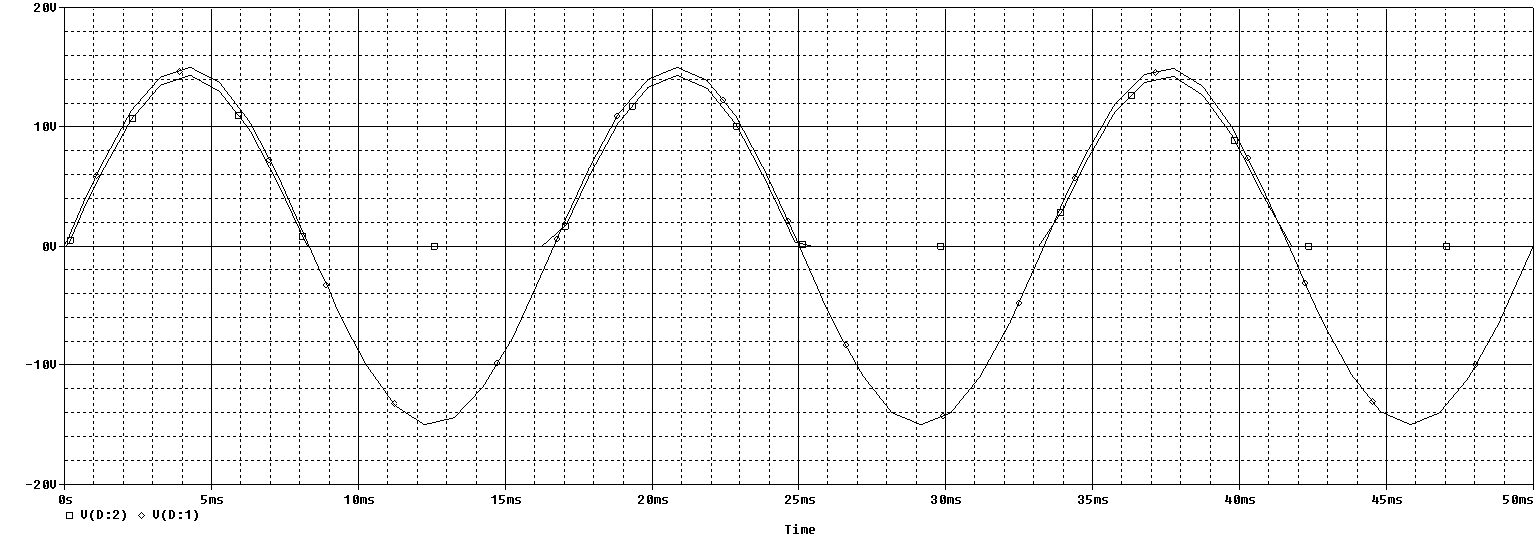
\includegraphics[width=1\textwidth]{graf210}
                \caption{Questão (1): tensão no resistor.}        
                \label{circ210}
            \end{figure}
            
            A partir destes valores e de \ref{eq:vp} é possível calcular o valor da capacitância \(C\) através da equação \ref{eq:ret1}, logo abaixo.
            
            \begin{equation} \label{eq:ret1}
            V_r = \frac{V_{p}}{fCR} \Rightarrow C = \frac{V_{p}}{fV_rR}
            \end{equation}
            
            Logo, calcula-se \(C= 104.90 ~\mu F\).
            
            O circuito, portanto, é representado pela figura~\ref{circ21}.
            
            \begin{figure}[h!] 
                \centering
                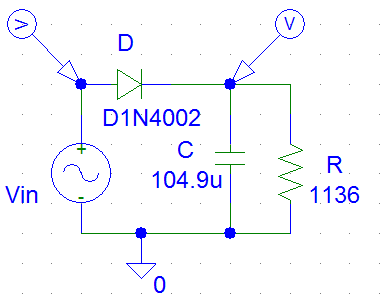
\includegraphics[width=0.250\textwidth]{circ21}
                \caption{Questão (1): retificador com capacitor.}        
                \label{circ21}
            \end{figure}

            Uma simulação do transitório desse circuito nos fornece o gráfico da figura~\ref{graf21}.
            
            \begin{figure}[h!] 
                \centering
                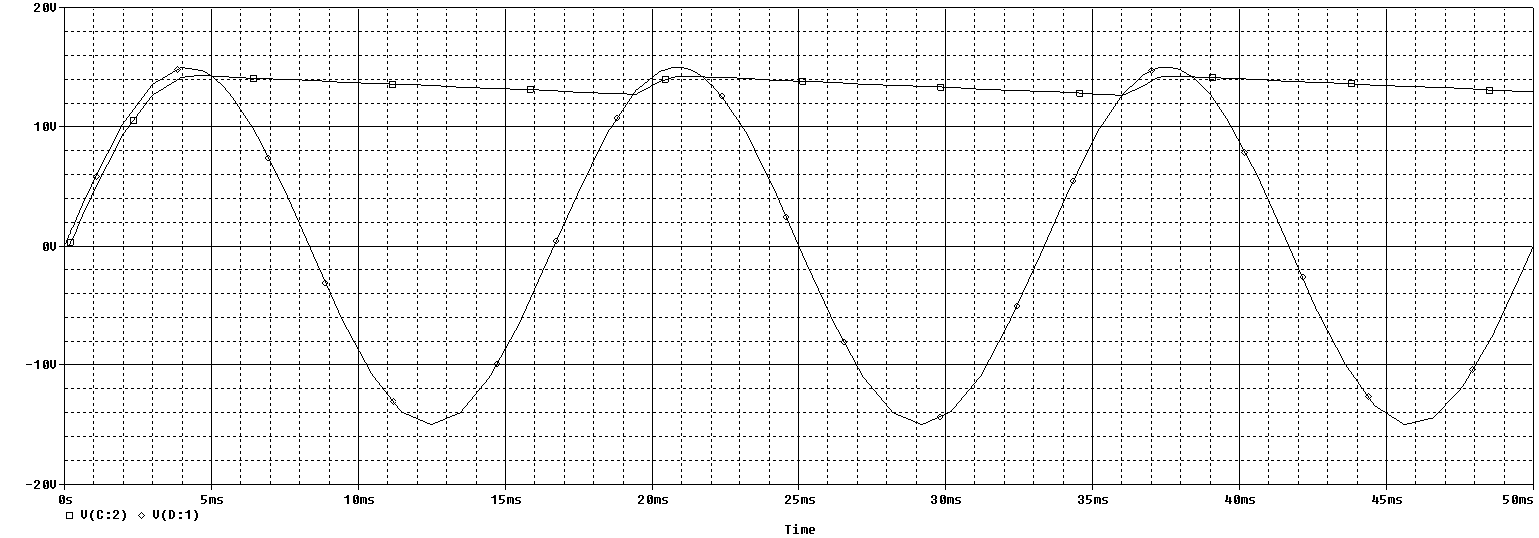
\includegraphics[width=1\textwidth]{graf21}
                \caption{Questão (1): tensões de entrada e saída.}        
                \label{graf21}
            \end{figure}
            
            Conforme esperado, o comportamento da tensão de saída aproxima-se do comportamento de uma tensão do tipo DC, isto é, de uma reta horizontal. As curvas, de aspecto exponencial e que dependem da constante de tempo RC, entre os picos do gráfico da tensão de entrada correspondem aos processos de descarregamento do capacitor a cada semiciclo negativo, isto é, quando o diodo está polarizado reversamente. Vale lembrar que pelo fato de RC ser grande, a função exponencial adquire este aspecto horizontal representado na figura. Nos semiciclos positivos (diodo está polarizado diretamente), o capacitor é carregado novamente com mesma constante de tempo \(RC\).
            
            \item O circuito utilizado para retificar ondas de amplitudes inferiores a 0.7V está representado na figura \ref{circ22}, abaixo.
            
            \begin{figure}[h!] 
                \centering
                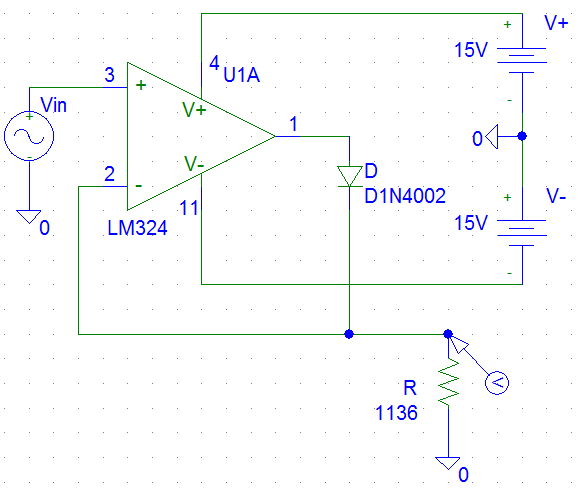
\includegraphics[width=0.30\textwidth]{circ22}
                \caption{Questão (2): retificador com com "superdiodo".}        
                \label{circ22}
            \end{figure}
            
            Na figura \ref{graf22}, tem-se o formato da onda da tensão de saída. Neste gráfico, é possível ver claramente a função do diodo. Nos semiciclos positivos, o diodo está polarizado diretamente, o que significa que o diodo permite a passagem de corrente e o amplificador operacional está sendo realimentado. Como consequência, existe entre os seus terminais a presença de um curto circuito virtual e, assim, \(v_{in} = v_{out}\). A tensão na saída do amplificador pode ser calculada através de \(v_d = v_{in} +0.7\), caso seja menor que a tensão de saturação. Nos semiciclos negativos,o diodo está reversamente polarizado, e, de maneira ideal, não permite passagem de corrente. Desta maneira, não há realimentação e nem curto virtual, resultando em \(v_{out} = 0\).
            
            \begin{figure}[h!] 
                \centering
                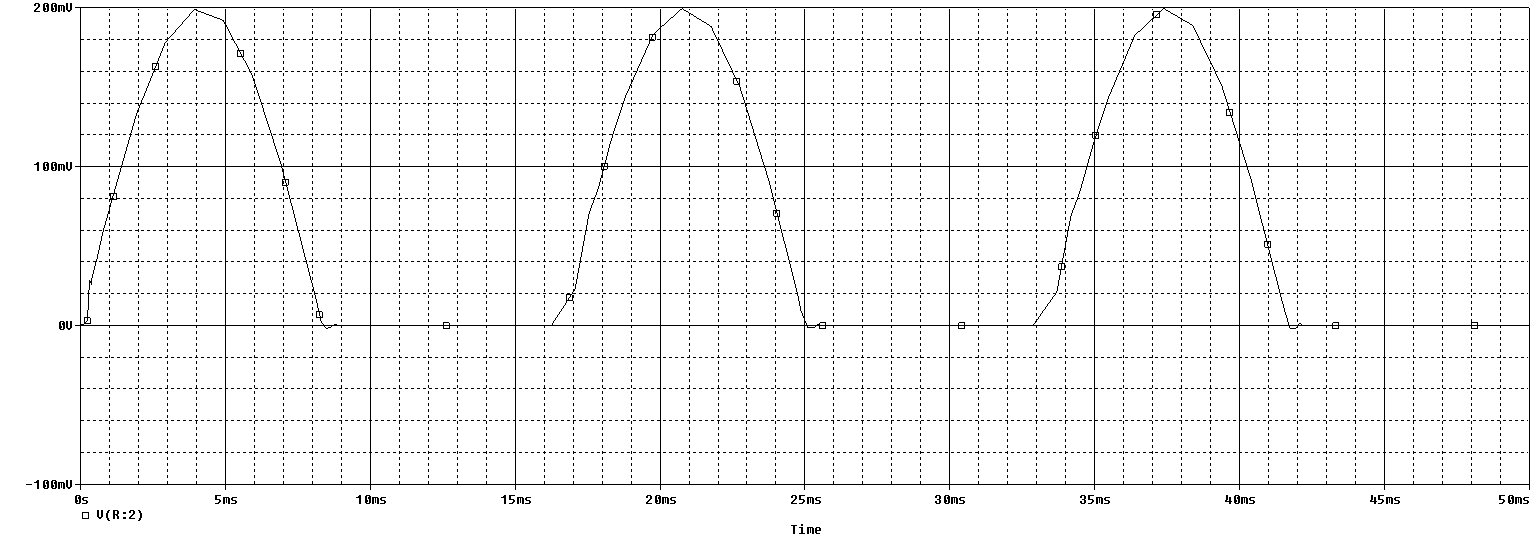
\includegraphics[width=1\textwidth]{graf22}
                \caption{Questão (2): tensão retificada de saída.}        
                \label{graf22}
            \end{figure}

            \item O circuito duplicador de voltagem está representado na figura \ref{circ23}.
            
            \begin{figure}[h!] 
                \centering
                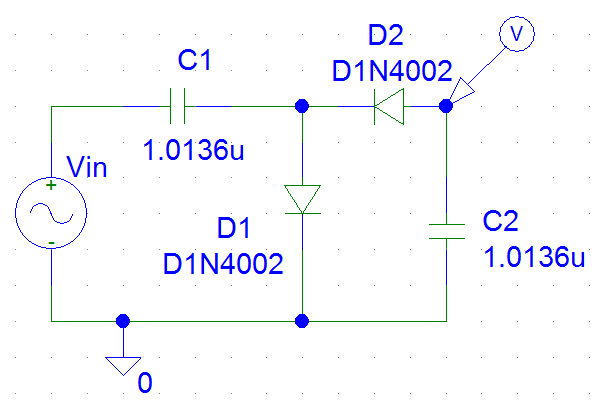
\includegraphics[width=0.30\textwidth]{circ23}
                \caption{Questão (3): circuito duplicador de voltagem.}        
                \label{circ23}
            \end{figure}
            
            A onda da tensão no diodo \(D_1\) simulada está no gráfico da figura \ref{graf231}. Conforme esperado, o pico máximo é aproximadamente 0V e o pico negativo é \(-2V_{in} = -30V\).
             
            \begin{figure}[h!] 
                \centering
                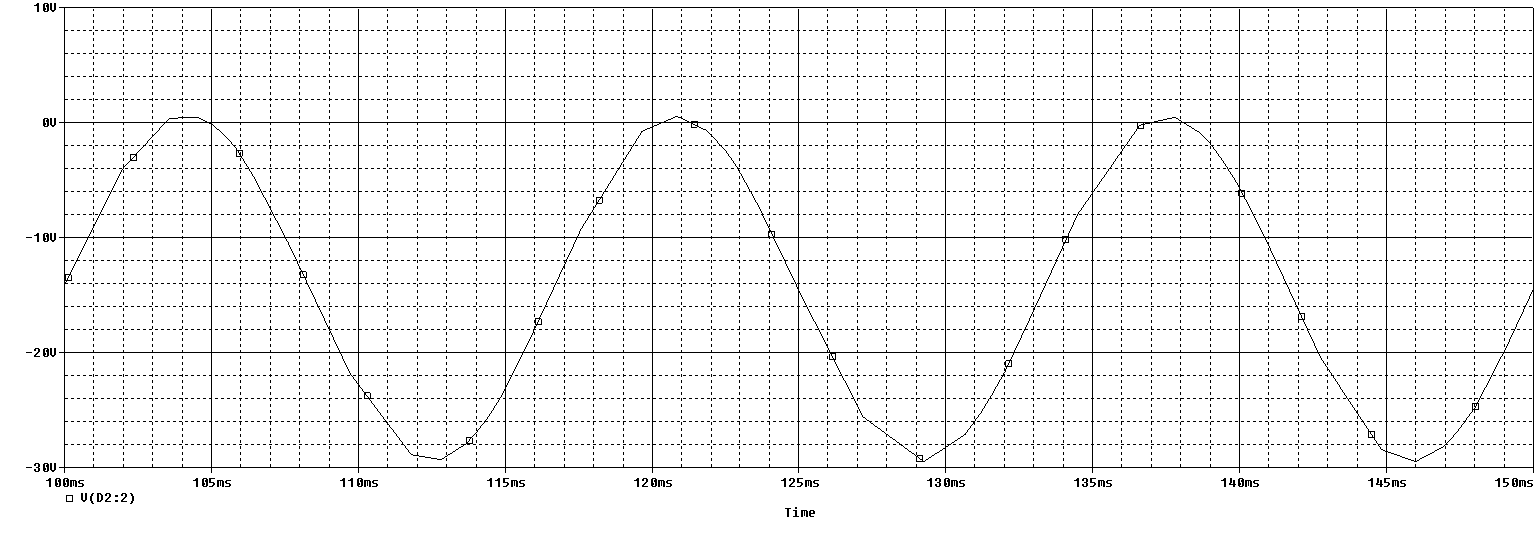
\includegraphics[width=1\textwidth]{graf231}
                \caption{Questão (3): tensão no diodo \(D_1\).}        
                \label{graf231}
            \end{figure}
            
            
            A tensão de saída está representada na figura \ref{graf232}. É possível visualizar que a partir de aproximadamente \(80ms\), a tensão de saída é constante e possui valor em torno de \(-2V_{in} = -30V\) e possui um comportamento DC.
            
            \begin{figure}[h!] 
                \centering
                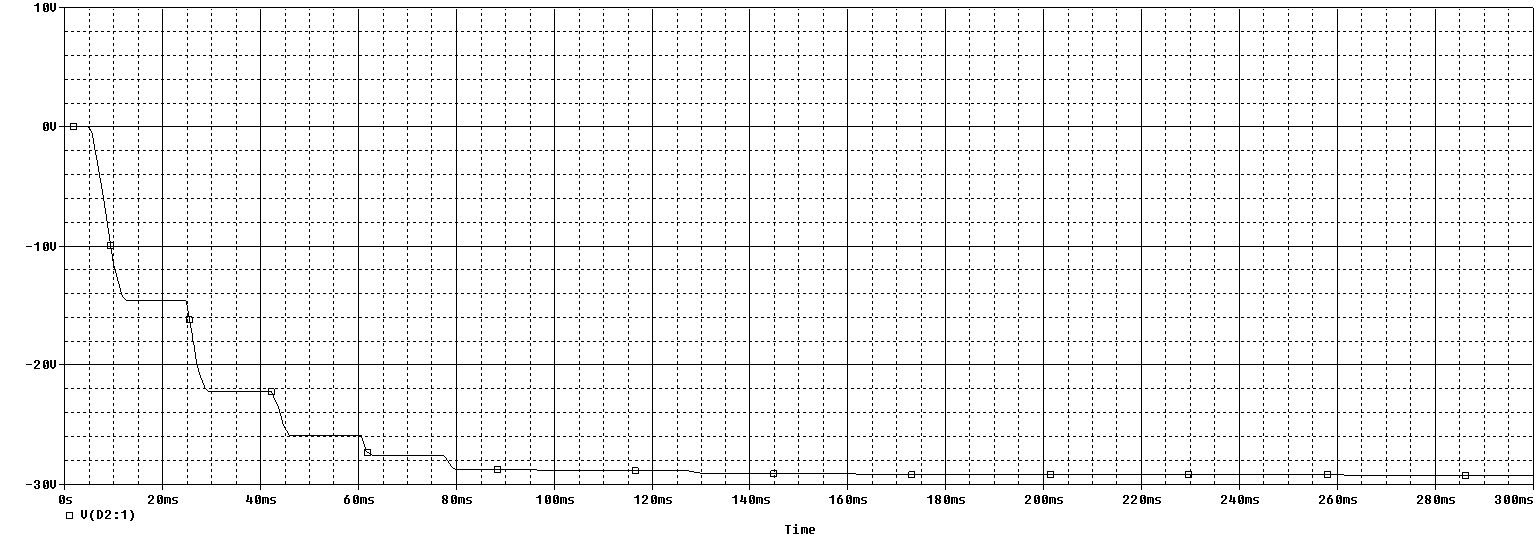
\includegraphics[width=1\textwidth]{graf232}
                \caption{Questão (3): tensão de saída.}        
                \label{graf232}
            \end{figure}
    \end{enumerate}

\end{document}